%% ----------------------------------------------------------------
%% Thesis.tex -- MAIN FILE (the one that you compile with LaTeX)
%% ---------------------------------------------------------------- 

% Set up the document
\documentclass[a4paper, 12pt, twoside]{Thesis}  % Use the "Thesis" style, based on the ECS Thesis style by Steve Gunn
\graphicspath{{Figures/}}  % Location of the graphics files (set up for graphics to be in PDF format)

% Include any extra LaTeX packages required
\usepackage[square, numbers, comma, sort&compress]{natbib}  % Use the "Natbib" style for the references in the Bibliography
\usepackage{verbatim}  % Needed for the "comment" environment to make LaTeX comments
\usepackage{vector}  % Allows "\bvec{}" and "\buvec{}" for "blackboard" style bold vectors in maths
\hypersetup{urlcolor=blue, colorlinks=true}  % Colours hyperlinks in blue, but this can be distracting if there are many links.

%% ----------------------------------------------------------------
\begin{document}
\frontmatter	  % Begin Roman style (i, ii, iii, iv...) page numbering

% Set up the Title Page
\title  {HTML5 WebSocket protocol and its application to distributed computing}
\authors  {Gabriel Muller}
\addresses  {\groupname\\\DEPTNAME\\\univname\\\coursename}  % Do not change this here, instead these must be set in the "Thesis.cls" file, please look through it instead
\date       {\today}
\subject    {}
\keywords   {}

\maketitle
\makesecondtitle
%% ----------------------------------------------------------------

\setstretch{1.3}  % It is better to have smaller font and larger line spacing than the other way round

% Define the page headers using the FancyHdr package and set up for one-sided printing
\fancyhead{}  % Clears all page headers and footers
\rhead{\thepage}  % Sets the right side header to show the page number
\lhead{}  % Clears the left side page header

\pagestyle{fancy}  % Finally, use the "fancy" page style to implement the FancyHdr headers

%% ----------------------------------------------------------------
% Declaration Page required for the Thesis, your institution may give you a different text to place here
\Declaration{

I, AUTHOR NAME, declare that this thesis titled, `THESIS TITLE' and the work presented in it are my own. I confirm that:

\begin{itemize} 
\item[\tiny{$\blacksquare$}] This work was done wholly or mainly while in candidature for a research degree at this University.
 
\item[\tiny{$\blacksquare$}] Where any part of this thesis has previously been submitted for a degree or any other qualification at this University or any other institution, this has been clearly stated.
 
\item[\tiny{$\blacksquare$}] Where I have consulted the published work of others, this is always clearly attributed.
 
\item[\tiny{$\blacksquare$}] Where I have quoted from the work of others, the source is always given. With the exception of such quotations, this thesis is entirely my own work.
 
\item[\tiny{$\blacksquare$}] I have acknowledged all main sources of help.
 
\item[\tiny{$\blacksquare$}] Where the thesis is based on work done by myself jointly with others, I have made clear exactly what was done by others and what I have contributed myself.
\\
\end{itemize}
 
 
Signed:\\
\rule[1em]{25em}{0.5pt}  % This prints a line for the signature
 
Date:\\
\rule[1em]{25em}{0.5pt}  % This prints a line to write the date
}
\clearpage  % Declaration ended, now start a new page

%% ----------------------------------------------------------------
% The "Funny Quote Page"
%\pagestyle{empty}  % No headers or footers for the following pages

%\null\vfill
% Now comes the "Funny Quote", written in italics
%\textit{``Write a funny quote here.''}

%\begin{flushright}
%If the quote is taken from someone, their name goes here
%\end{flushright}

%\vfill\vfill\vfill\vfill\vfill\vfill\null
%\clearpage  % Funny Quote page ended, start a new page
%% ----------------------------------------------------------------

% The Abstract Page
\chapter{Abstract}

The Thesis Abstract is written here (and usually kept to just this page). The page is kept centered vertically so can expand into the blank space above the title too\ldots


\clearpage  % Abstract ended, start a new page
%% ----------------------------------------------------------------

\setstretch{1.3}  % Reset the line-spacing to 1.3 for body text (if it has changed)

% The Acknowledgements page, for thanking everyone
\chapter{Acknowledgements}

The acknowledgements and the people to thank go here, don't forget to include your project advisor\ldots


\clearpage  % End of the Acknowledgements
%% ----------------------------------------------------------------

\pagestyle{fancy}  %The page style headers have been "empty" all this time, now use the "fancy" headers as defined before to bring them back


%% ----------------------------------------------------------------
\lhead{\emph{Contents}}  % Set the left side page header to "Contents"
\tableofcontents  % Write out the Table of Contents

%% ----------------------------------------------------------------
\lhead{\emph{List of Figures}}  % Set the left side page header to "List if Figures"
\listoffigures  % Write out the List of Figures

%% ----------------------------------------------------------------
\lhead{\emph{List of Tables}}  % Set the left side page header to "List of Tables"
\listoftables  % Write out the List of Tables

%% ----------------------------------------------------------------
\setstretch{1.5}  % Set the line spacing to 1.5, this makes the following tables easier to read
\clearpage  % Start a new page
\lhead{\emph{Abbreviations}}  % Set the left side page header to "Abbreviations"
\listofsymbols{ll}  % Include a list of Abbreviations (a table of two columns)
{
% \textbf{Acronym} & \textbf{W}hat (it) \textbf{S}tands \textbf{F}or \\
\textbf{LAH} & \textbf{L}ist \textbf{A}bbreviations \textbf{H}ere \\

}

%% ----------------------------------------------------------------
\clearpage  % Start a new page
\lhead{\emph{Physical Constants}}  % Set the left side page header to "Physical Constants"
\listofconstants{lrcl}  % Include a list of Physical Constants (a four column table)
{
% Constant Name & Symbol & = & Constant Value (with units) \\
Speed of Light & $c$ & $=$ & $2.997\ 924\ 58\times10^{8}\ \mbox{ms}^{-\mbox{s}}$ (exact)\\

}

%% ----------------------------------------------------------------
\clearpage  %Start a new page
\lhead{\emph{Symbols}}  % Set the left side page header to "Symbols"
\listofnomenclature{lll}  % Include a list of Symbols (a three column table)
{
% symbol & name & unit \\
$a$ & distance & m \\
$P$ & power & W (Js$^{-1}$) \\
& & \\ % Gap to separate the Roman symbols from the Greek
$\omega$ & angular frequency & rads$^{-1}$ \\
}
%% ----------------------------------------------------------------
% End of the pre-able, contents and lists of things
% Begin the Dedication page

\setstretch{1.3}  % Return the line spacing back to 1.3

\pagestyle{empty}  % Page style needs to be empty for this page
\dedicatory{For/Dedicated to/To my\ldots}

\addtocontents{toc}{\vspace{2em}}  % Add a gap in the Contents, for aesthetics


%% ----------------------------------------------------------------
\mainmatter	  % Begin normal, numeric (1,2,3...) page numbering
\pagestyle{fancy}  % Return the page headers back to the "fancy" style

% Include the chapters of the thesis, as separate files
% Just uncomment the lines as you write the chapters

% Chapter 1

\chapter{Chapter Title Here} % Write in your own chapter title
\label{Chapter1}
\lhead{Chapter 1. \emph{Chapter Title Here}} % Write in your own chapter title to set the page header


\section{Welcome and Thank You}

Welcome to this ``\LaTeX{} Thesis Template'', a beautiful and easy to use template for writing a thesis using the \LaTeX{} typesetting system.

If you are writing a thesis (or will be in the future) and its subject is technical or mathematical (though it doesn't have to be), then creating it in \LaTeX{} is highly recommended as a way to make sure you can just get down to the essential writing without having to worry over formatting or wasting time arguing with your word processor.

\LaTeX{} is easily able to professionally typeset documents that run to hundreds or thousands of pages long. With simple mark-up commands, it automatically sets out the table of contents, margins, page headers and footers and keeps the formatting consistent and beautiful. One of its main strengths is the way it can easily typeset mathematics, even \emph{heavy} mathematics. Even if those equations are the most horribly twisted and most difficult mathematical problems that can only be solved on a super-computer, you can at least count on \LaTeX{} to make them look stunning.

\subsection{Examples of \LaTeX{} Typeset eBooks}

You can see (and download and read) examples of eBooks typeset by \LaTeX{} in a small library here:\\
\href{http://www.sunilpatel.co.uk/typesetting.html}{\texttt{http://www.sunilpatel.co.uk/typesetting.html}}

The books are available for you to download for free. They were originally plain text files but were quickly and easily converted into beautifully typeset and well presented eBooks through \LaTeX{} for you to enjoy.


\section{Learning \LaTeX{}}

\LaTeX{} is not a WYSIWYG (What You See is What You Get) program, unlike word processors such as Microsoft Word or Corel WordPerfect. Instead, a document written for \LaTeX{} is actually a simple, plain text file that contains \emph{no formatting}. You tell \LaTeX{} how you want the formatting in the finished document by writing in simple commands amongst the text, for example, if I want to use \emph{italic text for emphasis}, I write the `$\backslash$\texttt{emph}\{\}' command and put the text I want in italics in between the curly braces. This means that \LaTeX{} is a ``mark-up'' language, very much like HTML.

\subsection{A (not so short) Introduction to \LaTeX{}}

If you are new to \LaTeX{}, there is a very good eBook -- freely available online as a PDF file -- called, ``The Not So Short Introduction to \LaTeX{}''. The book's title is typically shortened to just ``lshort''. You can download the latest version (as it is occasionally updated) from here:\\
\href{http://www.ctan.org/tex-archive/info/lshort/english/lshort.pdf}{\texttt{http://www.ctan.org/tex-archive/info/lshort/english/lshort.pdf}}

It is also available in several other languages. Find yours from the list on this page:\\
\href{http://www.ctan.org/tex-archive/info/lshort/}{\texttt{http://www.ctan.org/tex-archive/info/lshort/}}

It is recommended to take a little time out to learn how to use \LaTeX{} by creating several, small `test' documents. Making the effort now means you're not stuck learning the system when what you \emph{really} need to be doing is writing your thesis.

\subsection{A Short Math Guide for \LaTeX{}}

If you are writing a technical or mathematical thesis, then you may want to read the document by the AMS (American Mathematical Society) called, ``A Short Math Guide for \LaTeX{}''. It can be found online here:\\
\href{http://www.ams.org/tex/amslatex.html}{\texttt{http://www.ams.org/tex/amslatex.html}}\\
under the ``Additional Documentation'' section towards the bottom of the page.

\subsection{Common \LaTeX{} Math Symbols}
There are a multitude of mathematical symbols available for \LaTeX{} and it would take a great effort to learn the commands for them all. The most common ones you are likely to use are shown on this page:\\
\href{http://www.sunilpatel.co.uk/latexsymbols.html}{\texttt{http://www.sunilpatel.co.uk/latexsymbols.html}}

You can use this page as a reference or crib sheet, the symbols are rendered as large, high quality images so you can quickly find the \LaTeX{} command for the symbol you need.

\subsection{\LaTeX{} on a Mac}
 
The \LaTeX{} package is available for many systems including Windows, Linux and Mac OS X. The package for OS X is called MacTeX� and it contains all the applications you need � bundled together and pre-customised � for a fully working \LaTeX{} environment and work�ow.
 
MacTeX includes a dedicated \LaTeX{} IDE (Integrated Development Environment) called ``TeXShop'' for writing your `\texttt{.tex}' files and ``BibDesk'': a program to manage your references and create your bibliography section just as easily as managing songs and creating playlists in iTunes. To learn more about using \LaTeX{} on the Mac system, read the guide at:\\
\href{http://www.sunilpatel.co.uk/texhelp.html}{\texttt{http://www.sunilpatel.co.uk/texhelp.html }}


\section{Getting Started with this Template}

If you are familiar with \LaTeX{}, then you can familiarise yourself with the contents of the \href{http://www.sunilpatel.co.uk/files/Thesis\%20Template.zip}{Zip file} and the directory structure and then place your own information into the `\texttt{Thesis.cls}' file. Section \ref{FillingFile} on page \pageref{FillingFile} tells you how to do this. Make sure you read section \ref{ThesisConventions} about thesis conventions to get the most out of this template and then get started with the `\texttt{Thesis.tex}' file straightaway.

If you are new to \LaTeX{} it is recommended that you carry on reading through the rest of the information in this document.

\subsection{Latest Version}

This thesis template you have downloaded is version 1.2 and you can always find the latest version of this template online at:\\
\href{http://www.sunilpatel.co.uk/thesistemplate.html}{\texttt{http://www.sunilpatel.co.uk/thesistemplate.html}}

\subsection{List of Changes}

\subsubsection*{Version 1.2 (March 2008)}

This is version 1.2 and contains more corrections, improved advice on figures, an additional section for users on Mac systems and a major correction for those wishing to use US Letter sized paper for their thesis.

\subsubsection*{Version 1.1.2 (August 2007)}
This is version 1.1.2 and contains trivial (language and spelling) corrections.

\subsubsection*{Version 1.1.1 (May 2007)}
This is version 1.1.1 and corrects (updates) several hyperlinks that have changed. The file ``\texttt{lstpatch.sty}'' is also included as some \TeX{} distributions do not include it.

\subsubsection*{Version 1.1 (April 2007)}
This is version 1.1, released shortly after 1.0. It contains \emph{lots} of general text corrections (spelling, punctuation and grammar) and includes a link to a page containing a list of common \LaTeX{} math symbols, available at:\\
\href{http://www.sunilpatel.co.uk/latexsymbols.html}{\texttt{http://www.sunilpatel.co.uk/latexsymbols.html}}


\subsubsection*{Version 1.0 (March 2007)}
This is the first version, released to the public in March 2007.

\subsection{About this Template}

This \LaTeX{} Thesis Template is originally based and created around a \LaTeX{} style file created by Steve R.\ Gunn from the University of Southampton (UK), department of Electronics and Computer Science. You can find his original thesis style file at his site, here:\\
\href{http://www.ecs.soton.ac.uk/~srg/softwaretools/document/templates/}{\texttt{http://www.ecs.soton.ac.uk/$\sim$srg/softwaretools/document/templates/}}

My thesis originally used the `\texttt{ecsthesis.cls}' from his list of styles. However, I knew \LaTeX{} could still format better. To get the look I wanted, I modified his style and also created a skeleton framework and folder structure to place the thesis files in.

This Thesis Template consists of that modified style, the framework and the folder structure. All the work that has gone into the preparation and groundwork means that all you have to bother about is the writing.

Some of the modifications made to the original template include:
\begin{itemize}
\item Addition of the, `Declaration of Authorship' page
\item Optimised page layout for one-sided printing
\item Better page headers (changed from the default headers)
\item Full bibliography information (with `\texttt{natbib}' and `\texttt{unsrtnat}') that numerically sorts and compresses multiple references and also includes the URL field (with an active link) and DOI information if supplied
\item Change of font size and line spacing to increase readability
\item Added, `List of Symbols' page
\item Added, `funny quote' page
\end{itemize}


Before you begin using this template you should ensure that its style complies with the thesis style guidelines imposed by your institution. As this template is based on the style for the University of Southampton (UK), it can definitely be used without modification for Southampton PhD theses.

In most cases this template style and layout will be suitable. If it is not, it may only require a small change to bring the template in line with your institution's recommendations.


\section{What this Template Includes}

\subsection{Folders}

This template comes as a single \href{http://www.sunilpatel.co.uk/files/Thesis\%20Template.zip}{Zip file} that expands out to many files and folders. The folder names are mostly self-explanatory:

\textbf{Appendices} -- this is the folder where you put the appendices. Each appendix should go into its own separate `\texttt{.tex}' file.

\textbf{Chapters} -- this is the folder where you put the thesis chapters. A thesis usually has about seven chapters, though there is no hard rule on this. Each chapter should go in its own separate `\texttt{.tex}' file and they usually are split as:
\begin{itemize}
\item Chapter 1: Introduction to the thesis topic
\item Chapter 2: Background information and theory
\item Chapter 3: (Laboratory) experimental setup
\item Chapter 4: Details of experiment 1
\item Chapter 5: Details of experiment 2
\item Chapter 6: Discussion of the experimental results
\item Chapter 7: Conclusion and future directions
\end{itemize}
This chapter layout is specialised for the experimental sciences.

\textbf{Figures} -- this folder contains the all figures for the thesis. These are the final images that will go into the thesis document.

\textbf{Primitives} -- this is the folder that contains scraps, particularly because one final image in the `Figures' folder may be made from many separate images and photos, these source images go here. This keeps the intermediate files separate from the final thesis figures.

\subsection{Files}

Included are also several files, most of them are plain text and you can see their contents in a text editor. Luckily, many of them are auxiliary files created by \LaTeX{} or BibTeX and which you don't need to bother about:

\textbf{Bibliography.bib} -- this is an important file that contains all the bibliographic information and references that you will be citing in the thesis for use with BibTeX. You can write it manually, but there are reference manager programs available that will create and manage it for you. Bibliographies in \LaTeX{} are a large subject and you may need to read about BibTeX before starting with this.

\textbf{Thesis Todo List.txt} -- this is a Todo list that provides a simple way to track the thesis progress and also helps you see what parts need attention. Inside is a structured layout for you to enter all this information. Do not try to fill it out all at once, but write the tasks in as you come across them i.e.\ write an entry for a figure that needs creating only when you refer to or write about it (and hence need to place it) in the thesis text.

\textbf{Thesis.cls} -- this is an important file. It is the style file that tells \LaTeX{} how to format the thesis. You will also need to open this file in a text editor and fill in your own information (such as name, department, institution). Luckily, this is not too difficult and is explained in section \ref{FillingFile} on page \pageref{FillingFile}.

\textbf{Thesis.pdf} -- this is your beautifully typeset thesis (in the PDF file format) created by \LaTeX{}.

\textbf{Thesis.tex} -- this is an important file. This is the file that you tell \LaTeX{} to compile to produce your thesis as a PDF file. It contains the framework and constructs that tell \LaTeX{} how to layout the thesis. It is heavily commented so you can read exactly what each line of code does and why it is there. After you put your own information into the `\texttt{Thesis.cls}' file, go to this file and begin filling it in -- you have now started your thesis!

\textbf{vector.sty} -- this is a \LaTeX{} package, it tells \LaTeX{} how to typeset mathematical vectors. Using this package is very easy and you can read the documentation on the site (you just need to look at the `\texttt{vector.pdf}' file):\\
\href{http://www.ctan.org/tex-archive/macros/latex/contrib/vector/}{\texttt{http://www.ctan.org/tex-archive/macros/latex/contrib/vector/}}

\textbf{lstpatch.sty} -- this is a \LaTeX{} package required by this LaTeX template and is included as not all \TeX{} distributions have it installed by default. You do not need to modify this file.

Files that are \emph{not} included, but are created by \LaTeX{} as auxiliary files include:

\textbf{Thesis.aux} -- this is an auxiliary file generated by \LaTeX{}, if it is deleted \LaTeX{} simply regenerates it when you run the main `\texttt{.tex}' file.

\textbf{Thesis.bbl} -- this is an auxiliary file generated by BibTeX, if it is deleted, BibTeX simply regenerates it when you run the main tex file. Whereas the `\texttt{.bib}' file contains all the references you have, this `\texttt{.bbl}' file contains the references you have actually cited in the thesis and is used to build the bibliography section of the thesis.

\textbf{Thesis.blg} -- this is an auxiliary file generated by BibTeX, if it is deleted BibTeX simply regenerates it when you run the main `\texttt{.tex}' file.

\textbf{Thesis.lof} -- this is an auxiliary file generated by \LaTeX{}, if it is deleted \LaTeX{} simply regenerates it when you run the main `\texttt{.tex}' file. It tells \LaTeX{} how to build the `List of Figures' section.

\textbf{Thesis.log} -- this is an auxiliary file generated by \LaTeX{}, if it is deleted \LaTeX{} simply regenerates it when you run the main `\texttt{.tex}' file. It contains messages from \LaTeX{}, if you receive errors and warnings from \LaTeX{}, they will be in this `\texttt{.log}' file.

\textbf{Thesis.lot} -- this is an auxiliary file generated by \LaTeX{}, if it is deleted \LaTeX{} simply regenerates it when you run the main `\texttt{.tex}' file. It tells \LaTeX{} how to build the `List of Tables' section.

\textbf{Thesis.out} -- this is an auxiliary file generated by \LaTeX{}, if it is deleted \LaTeX{} simply regenerates it when you run the main `\texttt{.tex}' file.


So from this long list, only the files with the `\texttt{.sty}', `\texttt{.bib}', `\texttt{.cls}' and `\texttt{.tex}' extensions are the most important ones. The other auxiliary files can be ignored or deleted as \LaTeX{} and BibTeX will regenerate them.


\section{Filling in the `\texttt{Thesis.cls}' File}\label{FillingFile}

You will need to personalise the thesis template and make it your own by filling in your own information. This is done by editing the `\texttt{Thesis.cls}' file in a text editor.

Open the file and scroll down, past all the `$\backslash$\texttt{newcommand}\ldots' items until you see the entries for `\texttt{University Name}', `\texttt{Department Name}', etc\ldots.

Fill out the information about your group and institution and ensure you keep to block capitals where it asks you to. You can also insert web links, if you do, make sure you use the full URL, including the `\texttt{http://}' for this.

The last item you should need to fill in is the Faculty Name (in block capitals). When you have done this, save the file and recompile `\texttt{Thesis.tex}'. All the information you filled in should now be in the PDF, complete with web links. You can now begin your thesis proper!


\section{The `\texttt{Thesis.tex}' File Explained}

The \texttt{Thesis.tex} file contains the structure of the thesis. There are plenty of written comments that explain what pages, sections and formatting the \LaTeX{} code is creating. Initially there seems to be a lot of \LaTeX{} code, but this is all formatting, and it has all been taken care of so you don't have to do it.

Begin by filling out your information for the title page. For the thesis declaration, your institution may insist on something different than the text given. If this is the case, just replace what you see with what is required.

Then comes a page which contains a funny quote. You can put your own, or quote your favourite scientist, author, person, etc\ldots Make sure to put the name of the person who you took the quote from.

Next comes the acknowledgements. On this page, write about all the people who you wish to thank (not forgetting parents, partners and your advisor/supervisor).

The contents pages, list of figures and tables are all taken care of for you and do not need manually creating or editing. The next set of pages are optional and can be deleted since they are for a more technical thesis: Insert a list of abbreviations you have used in the thesis, then a list of the physical constants and numbers you refer to and finally, a list of mathematical symbols used in any formulae. Making the effort to fill these tables means the reader has a one-stop place to refer to instead of searching the internet and references to try and find out what you meant by certain abbreviations or symbols.

The list of symbols is split into the Roman and Greek alphabets. Whereas the abbreviations and symbols ought to be listed in alphabetical order (and this is \emph{not} done automatically for you) the list of physical constants should be grouped into similar themes.

The next page contains a one line dedication. Who will you dedicate your thesis to?

Finally, there is the section where the chapters are included. Uncomment the lines (delete the `\texttt{\%}' character) as you write the chapters. Each chapter should be written in its own file and put into the `Chapters' folder and named `\texttt{Chapter1}', `\texttt{Chapter2}, etc\ldots Similarly for the appendices, uncomment the lines as you need them. Each appendix should go into its own file and placed in the `Appendices' folder.

After the preamble, chapters and appendices finally comes the bibliography. The bibliography style (called `\texttt{unsrtnat}') is used for the bibliography and is a fully featured style that will even include links to where the referenced paper can be found online. Do not under estimate how grateful you reader will be to find that a reference to a paper is just a click away. Of course, this relies on you putting the URL information into the BibTeX file in the first place.

\section{Thesis Features and Conventions}\label{ThesisConventions}

To get the best out of this template, there are a few conventions that you may want to follow.

One of the most important (and most difficult) things to keep track of in such a long document as a thesis is consistency. Using certain conventions and ways of doing things (such as using the Todo list) makes the job easier. Of course, all of these are optional and you can adopt your own method.

\subsection{Printing Format}

This thesis template is designed for single sided printing as most theses are printed and bound this way. This means that the left margin is always wider than the right (for binding). Four out of �ve people will now judge the margins by eye and think, ``I never 
noticed that before.''.

The headers for the pages contain the page number on the right side (so it is easy to flick through to the page you want) and the chapter name on the left side.

The text is set to 11 point and a line spacing of 1.3. Generally, it is much more readable to have a smaller text size and wider gap between the lines than it is to have a larger text size and smaller gap. Again, you can tune the text size and spacing should you want or need to. The text size can be set in the options for the `$\backslash$\texttt{documentclass}' command at the top of the `\texttt{Thesis.tex}' file and the spacing can be changed by setting a different value in the `$\backslash$\texttt{setstretch}' commands (scattered throughout the `\texttt{Thesis.tex}' file).

\subsection{Using US Letter Paper}

The paper size used in the template is A4, which is a common � if not standard � size in Europe. If you are using this thesis template elsewhere and particularly in the United States, then you may have to change the A4 paper size to the US Letter size. Unfortunately, this is not as simple as replacing instances of `\texttt{a4paper}' with `\texttt{letterpaper}'.

This is because the final PDF file is created directly from the \LaTeX{} source using a program called `\texttt{pdfTeX}' and in certain conditions, paper size commands are ignored and all documents are created with the paper size set to the size stated in the configuration file for pdfTeX (called `\texttt{pdftex.cfg}').

What needs to be done is to change the paper size in the con�guration file for \texttt{pdfTeX} to reflect the letter size. There is an excellent tutorial on how to do this here: \\
\href{http://www.physics.wm.edu/~norman/latexhints/pdf_papersize.html}{\texttt{http://www.physics.wm.edu/$\sim$norman/latexhints/pdf\_papersize.html}}

It may be sufficient just to replace the dimensions of the A4 paper size with the US Letter size in the \texttt{pdftex.cfg} file. Due to the differences in the paper size, the resulting margins may be different to what you like or require (as it is common for Institutions to dictate certain margin sizes). If this is the case, then the margin sizes can be tweaked by opening up the \texttt{Thesis.cls} file and searching for the line beginning with, `$\backslash$\texttt{setmarginsrb}' (not very far down from the top), there you will see the margins speci�ed. Simply change those values to what you need (or what looks good) and save. Now your document should be set up for US Letter paper size with suitable margins.

\subsection{References}

The `\texttt{natbib}' package is used to format the bibliography and inserts references such as this one.\citep{Reference3} The options used in the `\texttt{Thesis.tex}' file mean that the references are listed in numerical order as they appear in the text. Multiple references are rearranged in numerical order\citep{Reference2, Reference1} and multiple, sequential references become reformatted to a reference range.\citep{Reference2, Reference1, Reference3} This is done automatically for you. To see how you use references, have a look at the `\texttt{Chapter1.tex}' source file.

References should come \emph{after} the punctuation mark if there is one (such as a comma or full stop). On the other hand, footnotes\footnote{Such as this footnote, here down at the bottom of the page.} come \emph{before} the punctuation mark. You can swap these around but the most important thing is to keep the convention consistent throughout the thesis. Footnotes themselves should be full, descriptive sentences (beginning with a capital letter and ending with a full stop).

To see how \LaTeX{} typesets the bibliography, have a look at the very end of this document (or just click on the reference number links).

\subsection{Figures}

There will hopefully be many figures in your thesis (that should be placed in the `Figures' folder). The way to insert figures into your thesis is to use a code template like this:
\begin{verbatim}
\begin{figure}[htbp]
  \centering
    \includegraphics{./Figures/Electron.pdf}
    \rule{35em}{0.5pt}
  \caption[An Electron]{An electron (artist's impression).}
  \label{fig:Electron}
\end{figure}
\end{verbatim}
Also look in the source file. Putting this code into the source file produces the picture of the electron that you can see in the figure below.

\begin{figure}[htbp]
	\centering
		\includegraphics{./Figures/Electron.pdf}
		\rule{35em}{0.5pt}
	\caption[An Electron]{An electron (artist's impression).}
	\label{fig:Electron}
\end{figure}

Sometimes figures don't always appear where you write them in the source. The placement depends on how much space there is on the page for the figure. Sometimes there is not enough room to fit a figure directly where it should go (in relation to the text) and so \LaTeX{} puts it at the top of the next page. Positioning figures is the job of \LaTeX{} and so you should only worry about making them look good!

Figures usually should have labels just in case you need to refer to them (such as in figure \ref{fig:Electron}). The `$\backslash$\texttt{caption}' command contains two parts, the first part, inside the square brackets is the title that will appear in the `List of Figures', and so should be short. The second part in the curly brackets should contain the longer and more descriptive caption text.

The `$\backslash$\texttt{rule}' command is optional and simply puts an aesthetic horizontal line below the image. If you do this for one image, do it for all of them.

The \LaTeX{} Thesis Template is able to use figures that are either in the PDF or JPEG file format. It is recommended that you read this short guide on how to get the best out of figures in \LaTeX{}, available here:\\
\href{http://www.sunilpatel.co.uk/texhelp5.html}{\texttt{http://www.sunilpatel.co.uk/texhelp5.html}}

Though it is geared more towards users of Mac and OS X systems, much of the advice applies to creating and using figures in general. It also explains why the PDF file format is preferred in figures over JPEG.

\subsection{Typesetting mathematics}

If your thesis is going to contain heavy mathematical content, be sure that \LaTeX{} will make it look beautiful, even though it won't be able to solve the equations for you.

The ``Not So Short Introduction to \LaTeX{}'' (available \href{http://www.ctan.org/tex-archive/info/lshort/english/lshort.pdf}{here}) should tell you everything you need to know for most cases of typesetting mathematics. If you need more information, a much more thorough mathematical guide is available from the AMS called, ``A Short Math Guide to \LaTeX{}'' and can be downloaded from:\\
\href{ftp://ftp.ams.org/pub/tex/doc/amsmath/short-math-guide.pdf}{\texttt{ftp://ftp.ams.org/pub/tex/doc/amsmath/short-math-guide.pdf}}

There are many different \LaTeX{} symbols to remember, luckily you can find the most common symbols \href{http://www.sunilpatel.co.uk/latexsymbols.html}{here}. You can use the web page as a quick reference or crib sheet and because the symbols are grouped and rendered as high quality images (each with a downloadable PDF), finding the symbol you need is quick and easy.

You can write an equation, which is automatically given an equation number by \LaTeX{} like this:
\begin{verbatim}
\begin{equation}
E = mc^{2}
  \label{eqn:Einstein}
\end{equation}
\end{verbatim}

This will produce Einstein's famous energy-matter equivalence equation:
\begin{equation}
E = mc^{2}
\label{eqn:Einstein}
\end{equation}

All equations you write (which are not in the middle of paragraph text) are automatically given equation numbers by \LaTeX{}. If you don't want a particular equation numbered, just put the command, `$\backslash$\texttt{nonumber}' immediately after the equation.


\section{Sectioning and Subsectioning}

You should break your thesis up into nice, bite-sized sections and subsections. \LaTeX{} automatically builds a table of Contents by looking at all the `$\backslash$\texttt{chapter}$\{\}$', `$\backslash$\texttt{section}$\{\}$' and `$\backslash$\texttt{subsection}$\{\}$' commands you write in the source.

The table of Contents should only list the sections to three (3) levels. A `$\backslash$\texttt{chapter}$\{\}$' is level one (1). A `$\backslash$\texttt{section}$\{\}$' is level two (2) and so a `$\backslash$\texttt{subsection}$\{\}$' is level three (3). In your thesis it is likely that you will even use a `$\backslash$\texttt{subsubsection}$\{\}$', which is level four (4). Adding all these will create an unnecessarily cluttered table of Contents and so you should use the `$\backslash$\texttt{subsubsection$^{*}\{\}$}' command instead (note the asterisk). The asterisk ($^{*}$) tells \LaTeX{} to omit listing the subsubsection in the Contents, keeping it clean and tidy.


\section{In Closing}

You have reached the end of this mini-guide. You can now rename or overwrite this pdf file and begin writing your own `\texttt{Chapter1.tex}' and the rest of your thesis. The easy work of setting up the structure and framework has been taken care of for you. It's now your job to fill it out! If you use this Thesis template and this mini-guide helps you, please let me know\footnote{Email: \href{mailto:web@sunilpatel.co.uk}{web@sunilpatel.co.uk} all comments and suggestions, questions and errata are welcome.}.

Good luck and have lots of fun!

\begin{flushright}
Sunil Patel: \href{http://www.sunilpatel.co.uk}{www.sunilpatel.co.uk}
\end{flushright}
 % Introduction

%\chapter{Literrature review} 
\label{Chapter2} 
\lhead{Chapter 2.\emph{Literrature review}}

This second chapter studies research done around WebSockets. The first
section is about the implementation of WebSockets server, the second is about
scalability. \\

\section{Implementation}

As in any project, in order to avoid future technical problems, it is better to
first study similar projects. The goal of this implementation study is to find a
suitable language and possibly a good library to run the experiment.

\subsection{WebSocket server implementation}

In order to narrow the library study, first a language needs to be selected.

\textbf{Language Selection}

Choosing a language for a project is often a compromise between the programmer
development background and the necessity of the application. Furthermore,
WebSocket servers can be developped in almost any languages.\\

This subsection does not aim at giving a comprehensive comparaison of all
existing WebSocket friendly languages. Node.js seems to be the perfect
environment for this study, therefore other languages will deliberatly be left
apart and the focus will be on explaining why Node.js is appropriate.\\

Node.js was specially invented to create real-time websites with push
capabilities \citep{Reference35}. Most languages run parallel tasks by using
threads but threads are memory expensive. Node.js is fundamentally different,
it runs as a single non-blocking and event-driven loop by using asynchronous
call back loops \citep{Reference37}. For this reasons, compared to other
languages, Node.js performs significantly better in highly concurrent
environment.\\

Node.js has many real-time engines. The next step is to carefully make a choice
between ws, Socket.io and Engine.io.\\  

\textbf{WebSocket implementation selection}

Deniz Ozger article's for medium.com \citep{Reference36} is a comprehensive study
of node.js real-time engines.\\

Ws is a pure WebSocket implementation, therefore it is interesting for testing
purpose but seldom used in real life projects.  The main drawback is the
communication may not work in case the browser does not support WebSockets.\\

Socket.io has some appreciable features namely it's connection procedure. First
it tries to connect to a server via WebSocket, in case it fails it downgrades
until it founds a suitable protocol. Moreover it tries to reconnect sockets
when connections fail.\\ 

Engine.io is a lower library of Socket.io. The connection procedure is the
opposite to Socket.io though. It first establishes a long polling connection
and only later tries to upgrade it to a better transport protocol. Therefore it
is more reliable because it establishes less connection.\\

In conclusion, Node.js and its real-time library engine.io seems a good choice
for our experiment. However better perfomance could be reached using an
heterogeneous implementation.


\subsection{Heterogeneous implementation with OpenCL}

As suggest John Stone paper's title \texttt{OpenCL: A parallel programming standard
for heterogeneous computing systems} \citep{Reference5} OpenCL is unanimously
considered as the refetence for heterogenous computing.\\

Historically, the first technology to take advantage of the massive parallel
nature of GPUs was Open Graphic Library (OpenGL). OpenGL is an application
programming interface (API) for rendering 2D and 3D vector graphics. Through
the insertion of little pieces of C-like codes in shader, developpers soon
realized graphic processing units (GPUs) could also be used for general
programming. This became known as General Purpose computation on GPUs (GPGPU)
\citep{Reference5}.\\

However, shadders can only be modified so much. As the need for more complex
applications arose Apple proposed the Khronos Group to develop a more general
framework: OpenCL. OpenCL is a low-level API accelerating applications with
task-parallel or data-parallel computations in a heterogeneous computing
environment. Indeed OpenCL not only allows the usage of CPUs but also any
processing devices like GPUs, DSPs, accelerators and so on \citep{Reference5}.
If generally on desktop the diversity of processing devices is quite low, it is
the opposite for mobile. Embedded systems for real-time multimedia journal
published a paper \citep{Reference3} highlining the advantages of using OpenCl
in mobile browser.\\

OpenCL doesn't guarantee a particular kernel will achieve peak performance on
different architectures. The nature of the underlying hardware may induce
different programming strategies. Multi-core CPU architecture is definitely the
more popular. But the recent specification published by Khronos to take GPU
computing to the web is bound to raise programmers interest toward GPUs
architecture \citep{Reference30}.\\ 

\textbf{CPUs architecture}

Modern CPUs are typically composed of a few high-frequency processor cores.
CPUs perform well for a wide variety of applications, but they are optimal for
latency sensitive workloads with minimal parallelism. However, to increase
performance during arithmetic and multimedia workloads,  many CPUs also
incorporate small scale use of single instruction multiple data (SIMD).\\

\textbf{GPUs architecture}

Contemporary GPUs are composed of hundreds of processing units running at low
frequency. \\

As a result GPUs are able to execute tens of thousands of threads. It is this
ability which makes them so much more effective then CPUs in a highly parallel
environment. Some research even claim a speedup in the order of 200x over
JavaScript. \citep{Reference3}\\

The GPU processing units are typically organized in SIMD clusters controlled by
single instruction decoders, with shared access to fast on-chip caches and
shared memories. Massively parallel arithmetic-heavy hardware design enables
GPUs to achieve single-precision floating point arithmetic rates approaching 2
trillions of instructions per second (TFLOPS). \citep{Reference5}\\

Although GPUs are powerful computing devices, currently they still often
require to be managemed by a host CPU. Fortunately OpenCL is designed to be used in
heterogeneous environment. It abstracts CPUs and GPUs as “compute devices”.
This way, applications can query device attributes to determine the
properties of the available compute units and memory systems.
\citep{Reference5}\\

All the same, even if OpenCL's API hides the hardest part of parallel
programming a good understanding of the underlying memory model leads to more
efficient codding. Along with general advises on how to build an OpenCL
cluster, details about the memory model are given in the following paper:
\citep{Reference4}.\\

\textbf{Platform model}

CPU and GPU are called “compute devices”. A single host regroups one or more
compute devices and has its own memory. Each compute device is composed of one
or more cores also called “compute units”. Each compute unit has its own memory
and is divided into one or more SIMD threads or “processing elements” with its
own memory. \citep{Reference4}\\

\begin{figure}[H] \centering
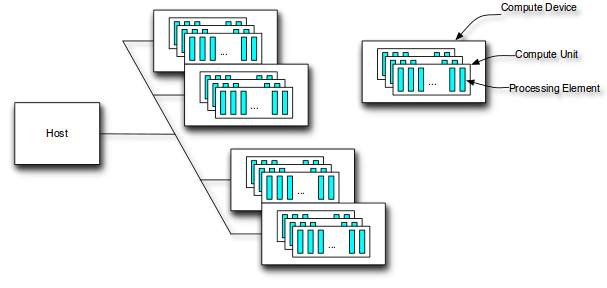
\includegraphics[width=\textwidth]{./Figures/plateform_model.png}
\caption[Plateform model]{Plateform model \citep{Reference4}}
\label{fig:plateform_model} \end{figure}


\textbf{Memory model}

OpenCL defines 4 types of memory spaces within a compute device. A large
high-latency “global” memory corresponding to the device RAM. This is a none
cached memory  where the data is stored and is available to all items. A small
low-latency read-only “constant” memory which is cached. A shared “local”
memory accessible from multiple processing elements within the same compute
unit and a “private” memory accessible within each processing element. This
last type of memory is very fast and is the register of the items
\citep{Reference4}.\\

\begin{figure}[H] \centering
  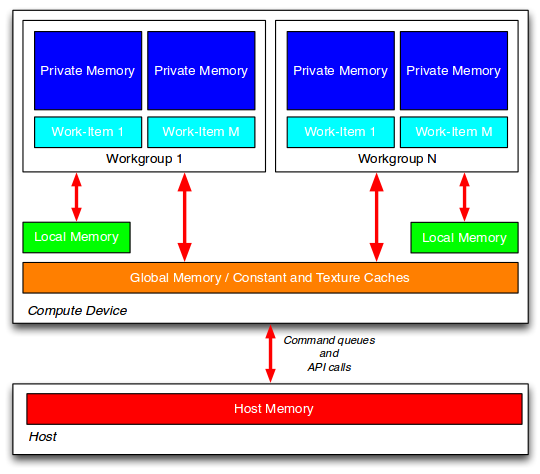
\includegraphics[width=0.6\textwidth]{./Figures/memory_model.png}
  \caption[Memory model]{Memory model \citep{Reference4}}
  \label{fig:memory_model} 
\end{figure}

In conclusion, OpenCL provides a fairly easy way to write parallel code but to
reach an optimal performance / memory access trade off programmers must choose
carefully in where to save their variables in memory space.\\

\textbf{Global and local IDs}

Finally, at an even lower level, work-items are scheduled in work–groups.
This is the smallest unit of parallelism on a device. Individual work-items in
a work–group  start together at the same program address, but they have their
own address counter and register state and are therefore free to branch and
execute independently \citep{Reference4}.\\

\begin{figure}[H] \centering
  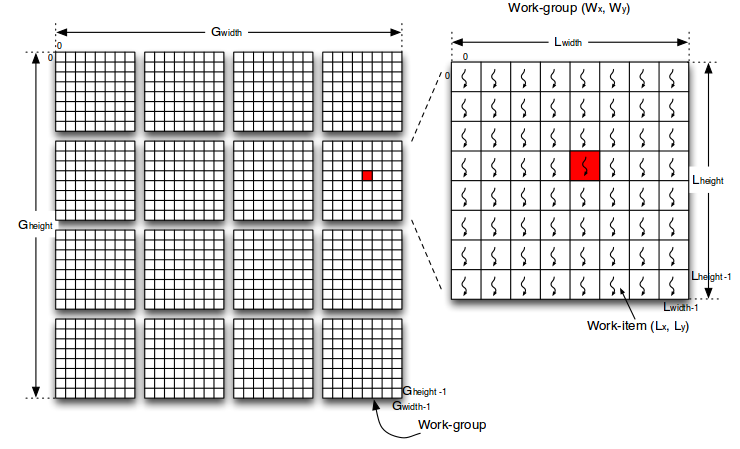
\includegraphics[width=\textwidth]{./Figures/id.png} 
  \caption[Work - group]{Work Group \citep{Reference4}} 
  \label{fig:id} 
\end{figure}


On a CPU, operating systems often swap two threads on and off execution
channels. Threads (cores ) are generally heavyweight entities and those context
switches are therefore expensive. By comparison, threads on a GPU ( work-items
) are extremely lightweight entities. Furthermore in GPUs, registers are
allocated to active threads only. Once threads are complete, its resources are
de-allocated.  Thus no swapping of registers or state occurs between GPU
threads. \citep{Reference4}\\

As can be deduced from this section about the underlying memory model, OpenCL is a
fairly low-level API. In fact, the programming language used is a derivate of
the C language based on C99. A language web developers will most likely be
unfamiliar with. Khronos anticipated this and developed the web computing
language (WebCL).\\

\subsection{WebCL}

WebGL and WebCL are JavaScript APIs over OpenGL and OpenCL's API. This allows
web developers to create application in an environment they are used to.\\

In the first place, OpenCL was developed because of web browser's increasing
need for more computational power. A necessity which arose from heavy 3D
graphics applications such as on-line games and augmented reality. However,
OpenCL doesn’t provide any rendering capability, it only processes huge amounts
of data. That is why OpenCL was designed for inter-operation with OpenGL.
WebCL/WebGL interoperability builds on that available for OpenCL/OpenGL. WebCL
provides an API for safely sharing buffers with OpenCL. This buffer is inside
the GPU which avoids the back and forth copy of data when switching between
OpenGL and OpenCL processes. Further precision about the interoperability are
discussed in this paper: \citep{Reference6}.\\

GPU computing is quite a new notion. But it is a fast evolving field of
research. Single GPUs are not enough anymore, the trend is moving towards GPU
clusters.\\

\subsection{GPU clusters}

Most OpenCL applications can utilize only devices of the hosting computer. In
order to run an application on a cluster, the program needs to be split to take
advantage of all devices. Virtual OpenCL (VirtualCL) is a wrapper for OpenCL.
It provides a platform where all the cluster devices are seen as if located on
the same hosting node. Basically, the user starts the application on the master
node then VirtualCL transparently runs the kernels of the application on the
worker nodes. Applications written with VirtualCL don't only benefit from the
reduced programming complexity of a single computer, but also from the
availability of shared memory and lower granularity parallelism. Mosix white
paper \citep{Reference7} explains more in depth the VCL's functionement.
\\

OpenCL and VirtualCL are powerful tool to create highly parallel clusters.  But
current implementation with CPUs only already reach a million concurrent
connections \citep{Reference13}. So far there is simply no need for more
powerful clusters.

However, all company don't have acccess to dual Quad-core Xeon CPUs used in
Kaazing cluster to reach a million concurrent connections. Usual practice is to
build a scalable cluster, to ajust computing power in fonction of the needs.

\section{Scalability}

The growth of distributed computing has changed the way web application are
designed and implemented. If compared with today standards, applications used
to be deployed so as to say at prototype stage. That is, they were designed to
work on a fixed number of servers and not able to ajust as the userbase grows.
As the number of connections increases, the load on the servers rises and thus
the latency grows. Ideally, an application should aim at a stabil latency,
otherwise the application can missbehave.\\ 

On the server side, the nodes will begin to be overloaded and struggle to
service the client with reasonable response time.\\ 

Also, if the servers are overwhelmed they buffer the responses to the clients
and then catch up later on . As a result, the clients can be flooded when the
load goes down. The sudden rush of message can provoke an unexpected behavior
from the servers and can even lead to disconnections.\\

Nowadays, designing an application without scalability and load balancing in
mind is unimaginable. Historically, the reaction to an overloaded server
has always been to scale up.\\

\subsection{Scaling up}

Scaling up or vertically basically means upgrading the infrastructure.
Depending on the needs of the application, the processor, the memory, the
storage or the network connectivity can be improved.\\

Further performance can be gained by dividing tasks. It only requires to
identify the services  running idependantly or the using message based
communication. Those could then be relocated on different nodes.\\

The main advantage of scaling vertically is it does not involve any software
changes and little infrastructure changes. Therefore it is an easy way to
increase performances. However for large application, scaling up might prove
impossible or at least not economicaly profitable. In case the infrastrucure 
is already equiped with the lastest hardware generation, the tiniest
increase in performance will impact greatly the price. For example, a high
range processor offering ten pourcent more computation power is going to be
many times more expensive. Similarly, a memory upgrade could require remplacing
all current modules for higher density ones.\\

Moreover, scaling up neither answers availability nor uptime concerns. The
system is monolithic and has a single point of failure. Therefore contemporary
project usually scale out and use parallel computing.\\

\subsection{Scaling out}
				
Scaling out or horizontally, answers most of the problems unsolved by scaling
vertically. In a first approach lets ignore the software complexity.  Scaling
out offers almost unlimitted performance increase and at low cost! If the
application is designed to be spread out on multiple nodes, the performance of
an infrastructure can be doubled by simply using twice as much servers. Also it
is fairly easy to add some redundant server to insure uptime. Plus, compared to
scaling up, once the sofware is developped the costs are linear.\\

When scaling out, the infrastructure implementation is not as much a problem as
the code implementation. The expenses are shifted from hardware to developpment
costs.\\

\textbf{Code implementation}

Developping a parallel code is quite complicated and all applications can not
be parallized. In 1967 Gene M. Amdhal defined the so called Amdahl's law which
is still used today to define the maximum to expect when parallelizing a code
\citep{Reference10}. \\

Each software can be divided in two separete parts, the parallel part and the
sequential part. Parallel computing does not improve the sequential part. If a
the code is mainly sequential, then increasing the number of processors will
only cause the parallel part to finish first and stay idle waiting for the
sequential part to finish.\\ 

Assuming P is the portion of a program that can be parallelized and 1 - P  is
the portion that remains serial, then the maximum speedup that can be achieved
using N processors is: 

$$speedup(N) = \frac{1}{(1-P) + \frac{P}{N}} $$

If 70\% of the program can be run in parallel (P = 0.7) the maximum expected
speedup with 4 processors would be:

$$speedup(N) = \frac{1}{(1-0.7) + \frac{0.7}{N}}$$

$$speedup(4) = 2.1$$

When the number of processors reaches a certain point, the speed up will be:


$$\lim\limits_{N \to \infty} speedup(N)= \frac{1}{1-P} = 3.3$$\\


Nathan T. Hayes's paper for Sunfish Studio \citep{Reference8} studies how
parallel computing can profit the motion picture industrie. The following chart
present the maximum speedup which can be expected from an application in
function of the pourcentage of parallel code in the programme.\\

\begin{figure}[H] 
  \centering
  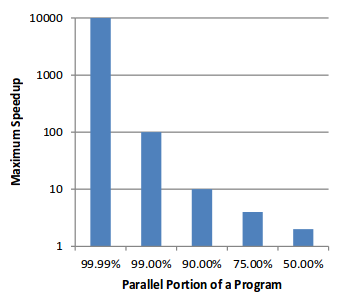
\includegraphics[width=0.5\textwidth]{./Figures/amdahl.png}
  \caption[Amdahl law]{Amdahl law \citep{Reference8}} 
  \label{fig:amdahl} 
\end{figure}

The figures speak for itslelf, to envisage parallel computing, the portion of
parallel code must be very high.

However, Amdahl's law is based on assumption which are hardly verified in
pratique. Following are sumed up reasons not to give to much importance to
Amdahl's law \citep{Reference34}:

\begin{itemize} 
  \item The number of thread is not always always equivalent to the number of processors.  
  \item The parallel portion does not have a perfect speedup. Computation power is used
    for communication between processus. Also some ressources like caches and bandwidth
    have to be shared across all the processors.  
  \item Allocating, delocating and switching threads introduce overhead, overhead growing
    linearly with the number of thread.  
  \item Even an optimized code will not have perfectly synchronised threads, at some point
    some processus will have to wait for others to finish.	
\end{itemize}


Amdahl's law has long been used as an argument against massively parallel
processing. In 1988 Gustafson law came as an alternative to Amdahl's law to
estimate the speedup. In both law, the sequential portion of the problem is
supposed to stay constant. But in Gustafson's law the overall problem size
grows proportionally to the number of cores. As a result, Gustafson's gives
slightly different results to Amdahl's and encourage the use of parallel
computing.\\

However later studies tends to contest the legimity of both laws. Yuan Shi's
paper \citep{Reference9} even proves both theory are but two different
interpretations of the same law. He concludes his study by saying these laws
are too minimalist and what computer scientist really need is a practical
engineering tool that can help the community to identify performance critical
factors.\\

\textbf{Infrastructure implementation}

Beside coding complication, scaling out also brings infrastructure changes.
A third party must be in command of all servers. This master server is also called
load balancer. Its role is to distribute the work evenly between the workers and thus
completly hides the complexity to the user.\\


 % Background Theory 

%\chapter{Experiment}
\label{Chapter3}
\lhead{Chapter 3. \emph{Experiment}}

\section{Client side}



 % Experimental Setup

%\chapter{Experiment} 
\label{Chapter4} 
\lhead{Chapter 4. \emph{Experiment}} 

\section{Client throughout}

\subsection{Client scalability}

SocketCluster-client makes the instanciation of a WebSocket clients on one core
quite straightforward. To deploy it on all available nodes, node.js
\texttt{fork()} function is used. A client code example is given in appendix
\ref{fig:WS_client_simplePing}.

The first experiment is a safety test. It checks if \texttt{fork()} distributes
evenly the work among the cores.

\begin{center}
  \begin{tabular}{ | l | l |}
  \hline
  \multicolumn{2}{|c|}{Parameters} \\
  \hline
    Instance type &  amazon s3 m3.2xlarge\\ 
    Experiment time & 120 s \\
    Number of new communication created at each iteration & 15 \\
    Client creation period & 1 s \\
    Type of ping & random number \\ 
    Ping period & 2.5 s \\ 
  \hline
  \end{tabular}
\end{center}

\begin{figure}[H]
	\centering
		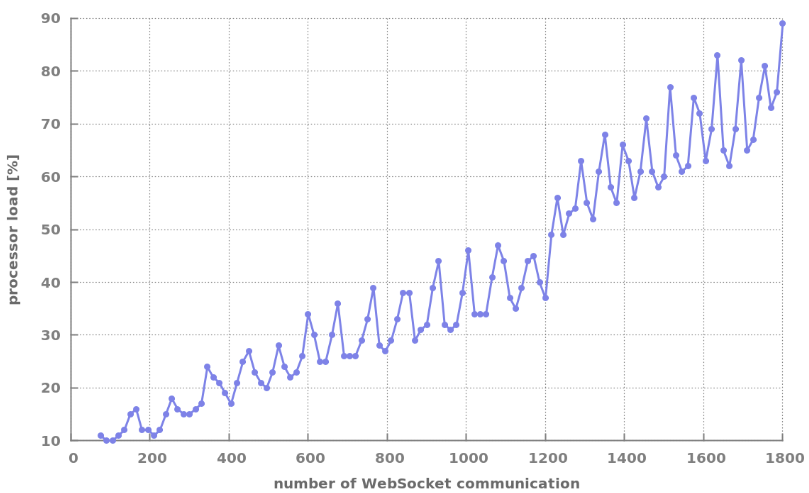
\includegraphics[width=\textwidth]{./Figures/1_client.png}
		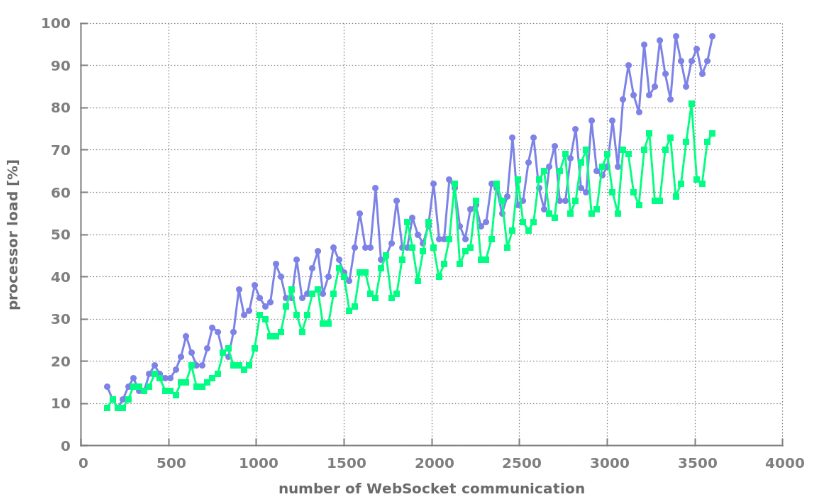
\includegraphics[width=\textwidth]{./Figures/2_client.png}
	\caption[Client throughout]{Client throughout}
	\label{fig:1+2_client}
\end{figure}


From figure \ref{fig:1+2_client} can be inferred that the client
implementation works flawlessly. Adding a second core enables twice as much
communication  to be established.

\subsection{browser testing}

As mentionned in appendix \ref{fig:index_script}, by opering minor changes in
the \texttt{index.html} file, the browser can be configured to display in real
time the number of pings received by a particular worker. If the experiment is
running locally, typing \texttt{localhost:8080} in the url will link the
browser to one worker.\\

\begin{figure}[H]
	\centering
		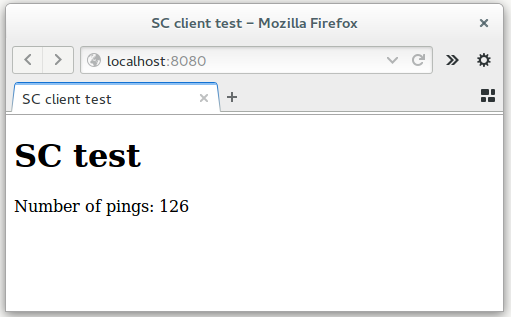
\includegraphics[width=0.9\textwidth]{./Figures/browser.png}
	\caption[Browser connection to SocketCluster]{Browser connection to SocketCluster}
	\label{fig:browser}
\end{figure}

By doing so we can embody a user connected to our WebSocket server and have a
better idea of the reactivity of the server.

% --------------
% second section
% --------------

\section{Comparaison with engine.io}

SocketCluster has been created to ease the creation of multi - core WebSocket
server. Logicaly the first experiment carried out on the server was to compare
a WebSocket to a traditionnal Engine.io server. 

Engine.io and SocketCluster codes can be found in appendix \ref{SocketCluster} and \ref{engine}. 

\begin{center}
  \begin{tabular}{ | l | l |}
  \hline
  \multicolumn{2}{|c|}{Parameters} \\
  \hline
    Instance type &  amazon ec2 m3.2xlarge\\ 
    Experiment time & 60 s \\
    Number of new communication created at each iteration & 20 \\
    Client creation period & 1 s \\
    Type of ping & random number \\ 
    Ping period & 2.5 s \\ 
    Number of clients & 2 \\
  \hline
  \end{tabular}
\end{center}


\begin{figure}[H]
	\centering
		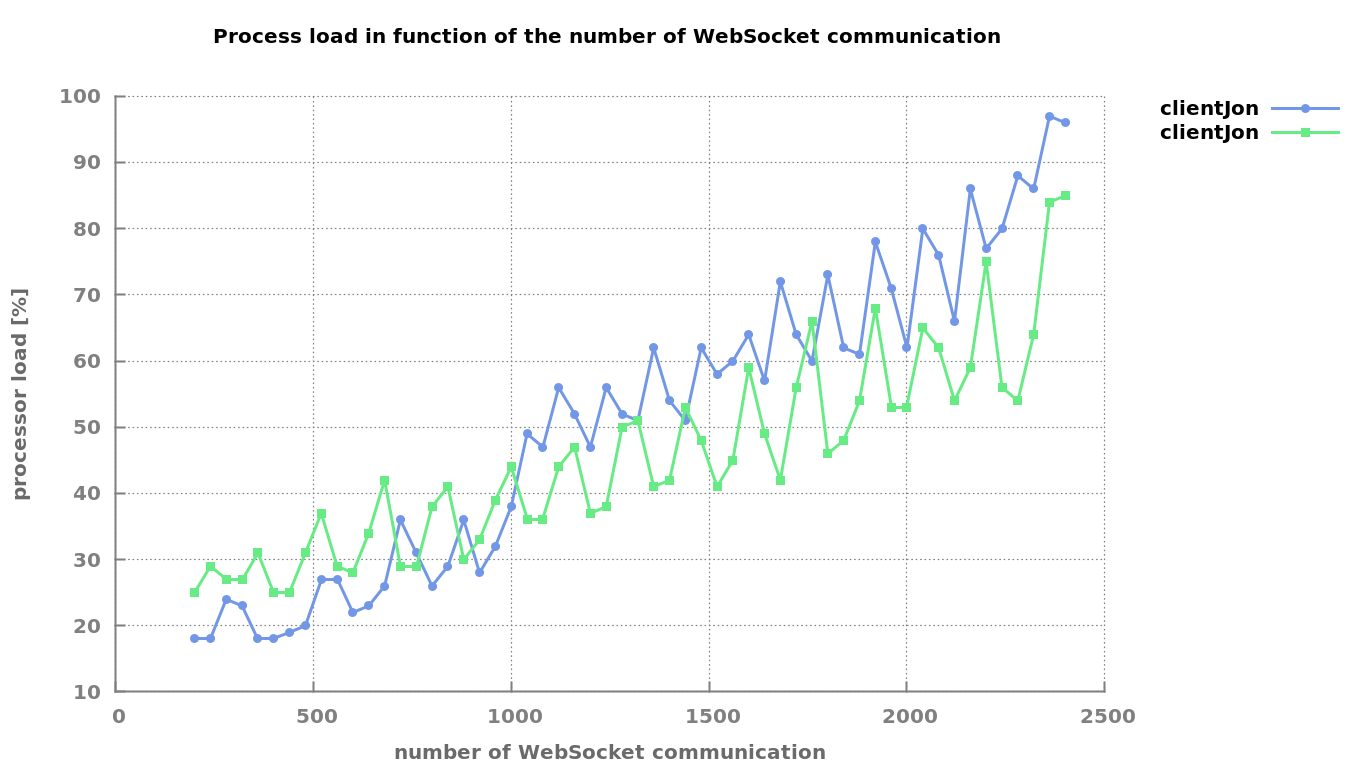
\includegraphics[width=\textwidth]{./Figures/WS_client_comparaison.png}
		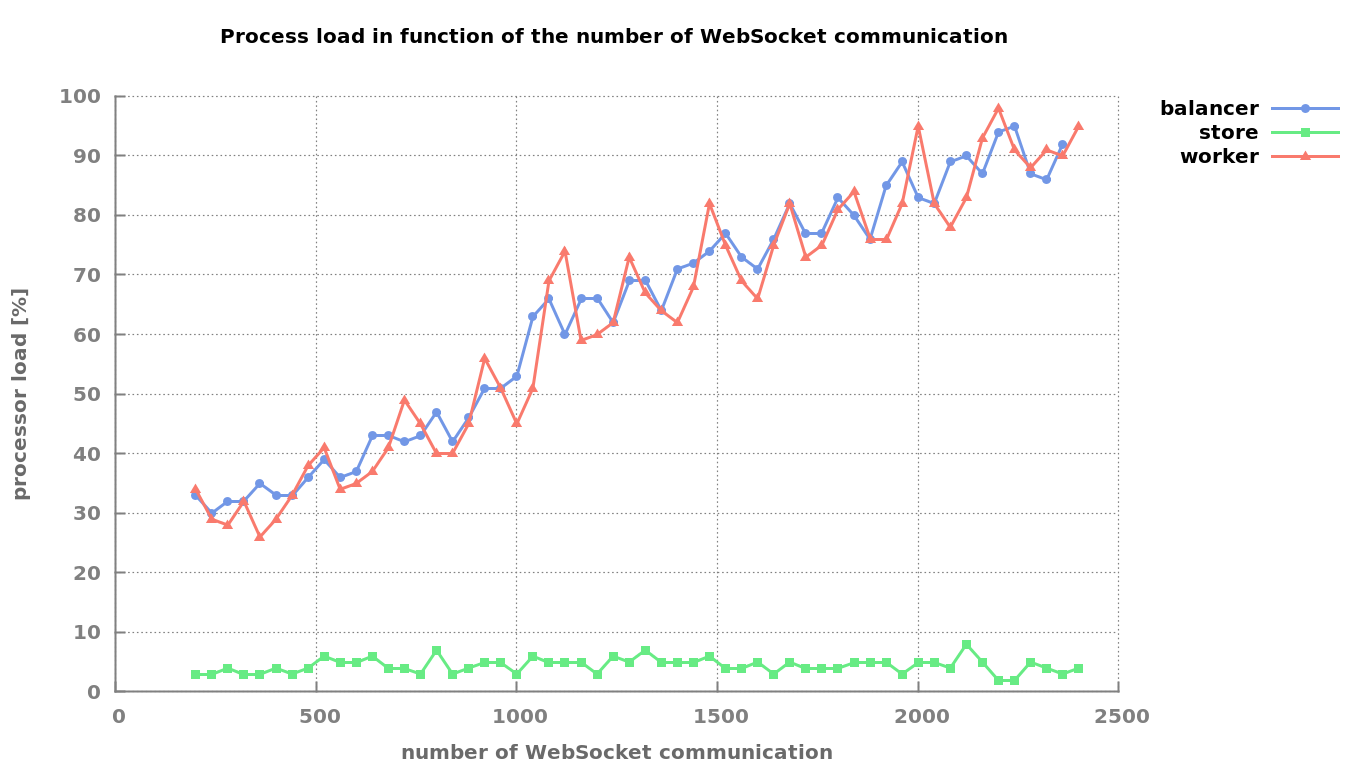
\includegraphics[width=\textwidth]{./Figures/WS_server_comparaison.png}
	\caption[WebSocket implementation]{WebSocket implementation}
	\label{fig:WS_comparaison}
\end{figure}

In this experience, two clients are used to achieve a maximum of 2400 WebSocket
communications.  The server was configured to use one storage, one load
balancer and one worker. While the store processor is quite idle, the two other
processors on the other hand are almost used at full capacity.

\begin{figure}[H]
	\centering
		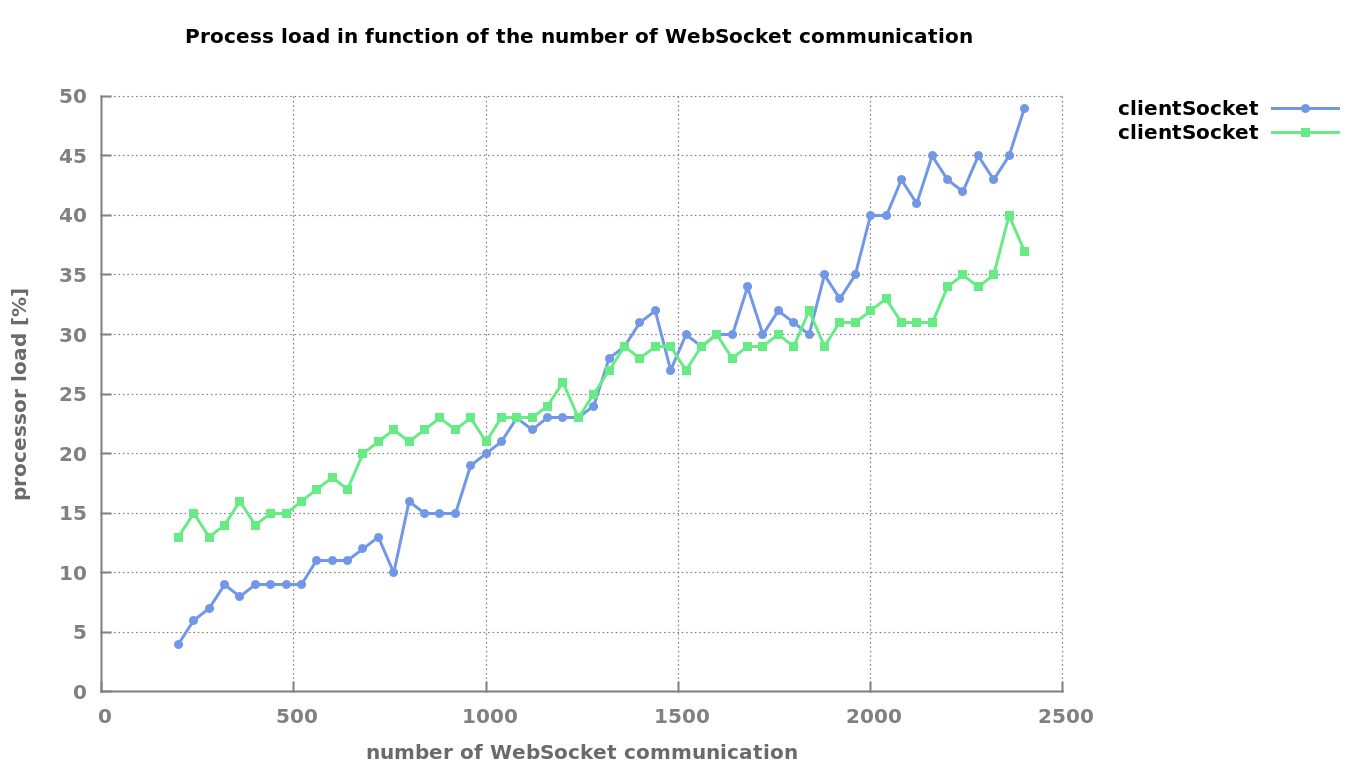
\includegraphics[width=\textwidth]{./Figures/engine_client_comparaison.png}
		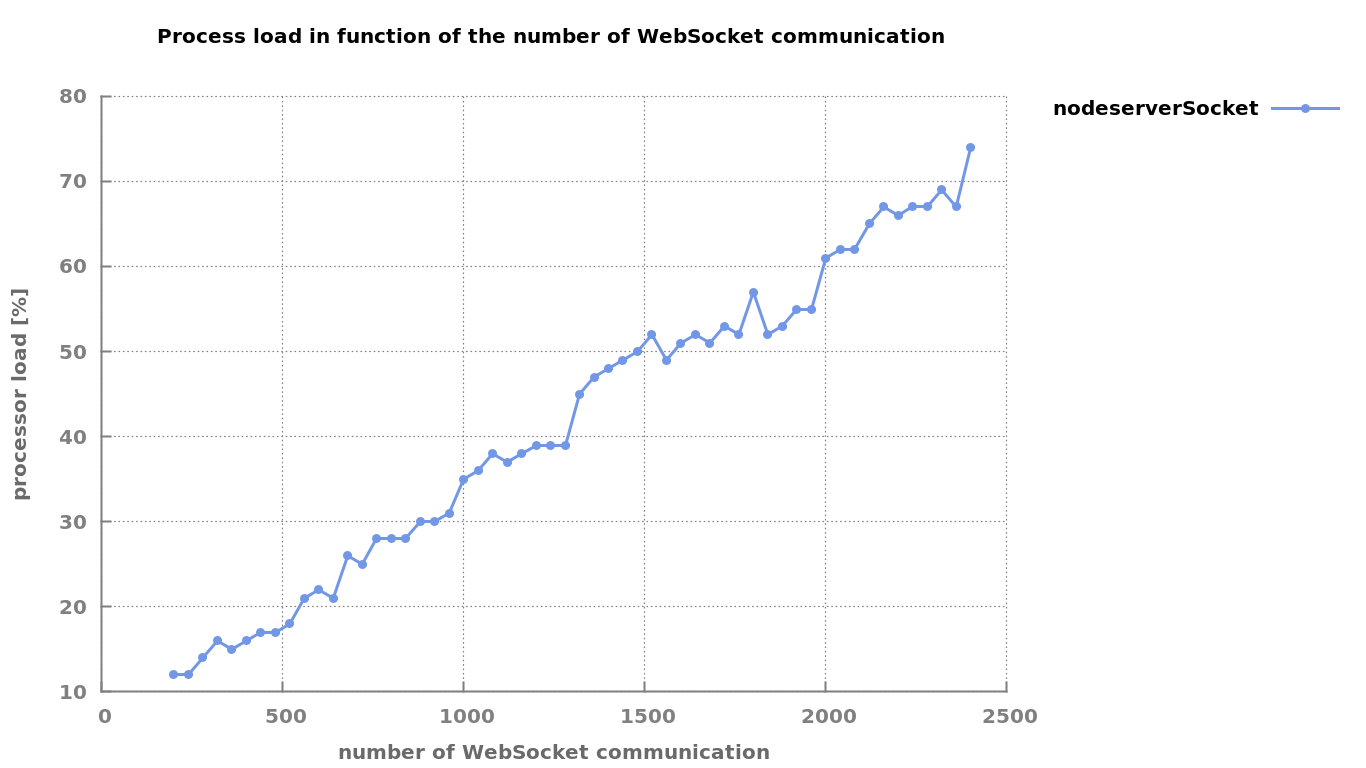
\includegraphics[width=\textwidth]{./Figures/engine_server_comparaison.png}
	\caption[Engine.io implementation]{Engine.io implementation}
	\label{fig:engine_comparaison}
\end{figure}

Surprisingly, pure engine.io implementation seems to be more efficient. Clients
are hitting a maximum of 50\% processor usage compared to 90\% for WebSockets.

On the server side also, engine.io processor peaks at 75\% compared to almost
100\% for WebSockets. Also even if both code have been deployed on similar
virtual machines: \texttt{amazon ec2 m3.2xlarge} the engine.io server is
running only only on one core compared to three for SocketCluster (one storage,
one load balancer and one worker). This seems to show, SocketCluster is not
adapted to low number of communication.

An interesting experiment worth doing at this point, is to try to use
SocketCluster on one core.

% -------------
% Third section
% -------------

\section{SocketCluster context switching}

For this experiment a single core  virtual machine is used for the server:
\texttt{amazon ec2 m3.medium}.

\begin{center}
  \begin{tabular}{ | l | l |}
  \hline
  \multicolumn{2}{|c|}{Parameters} \\
  \hline
    Server instance type &  amazon ec2 m3.medium\\ 
    Client instance type &  amazon ec2 m3.2xlarge\\
    Experiment time & 80 s \\
    Number of new communication created at each iteration & 40 \\
    Client creation period & 1 s \\
    Type of ping & random number \\ 
    Ping period & 2.5 s \\ 
    Number of clients & 2 \\
  \hline
  \end{tabular}
\end{center}

\begin{figure}[H]
	\centering
		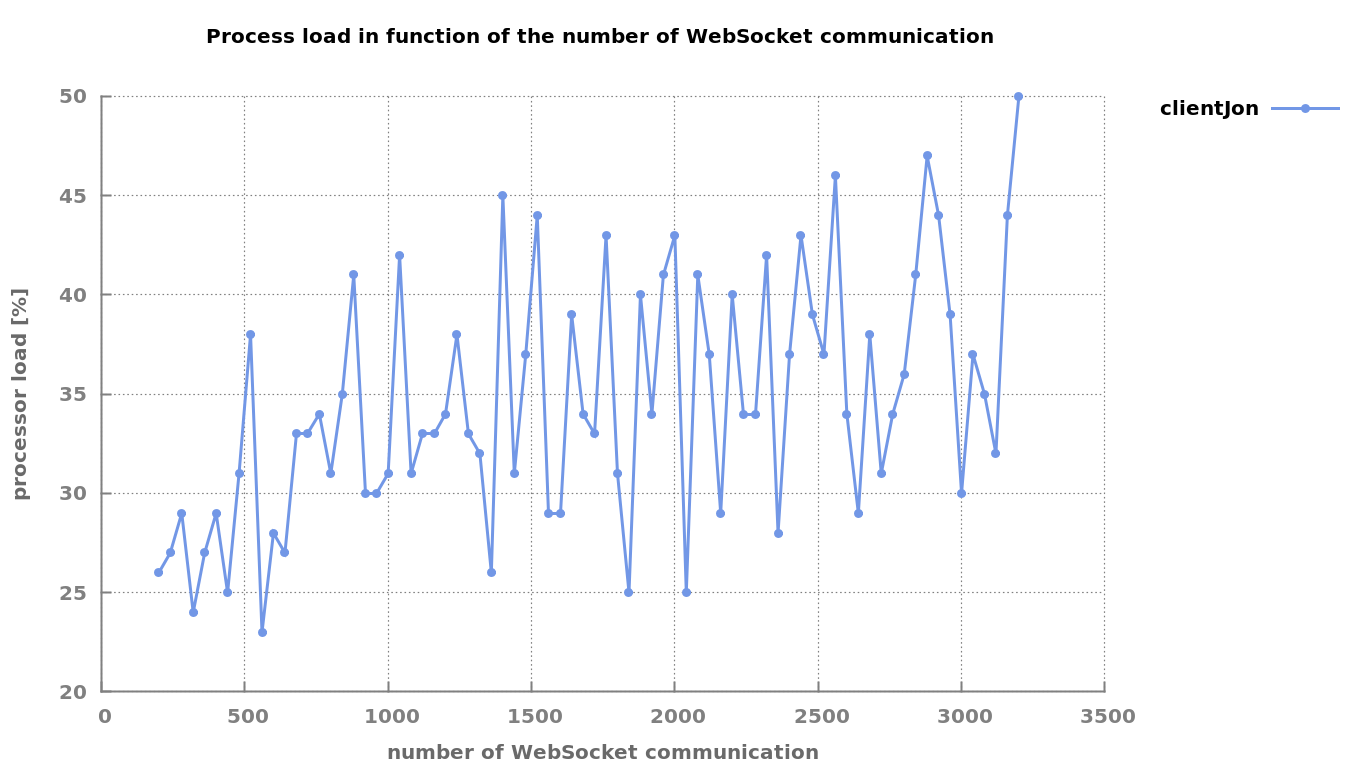
\includegraphics[width=\textwidth]{./Figures/WS_client_context.png}
		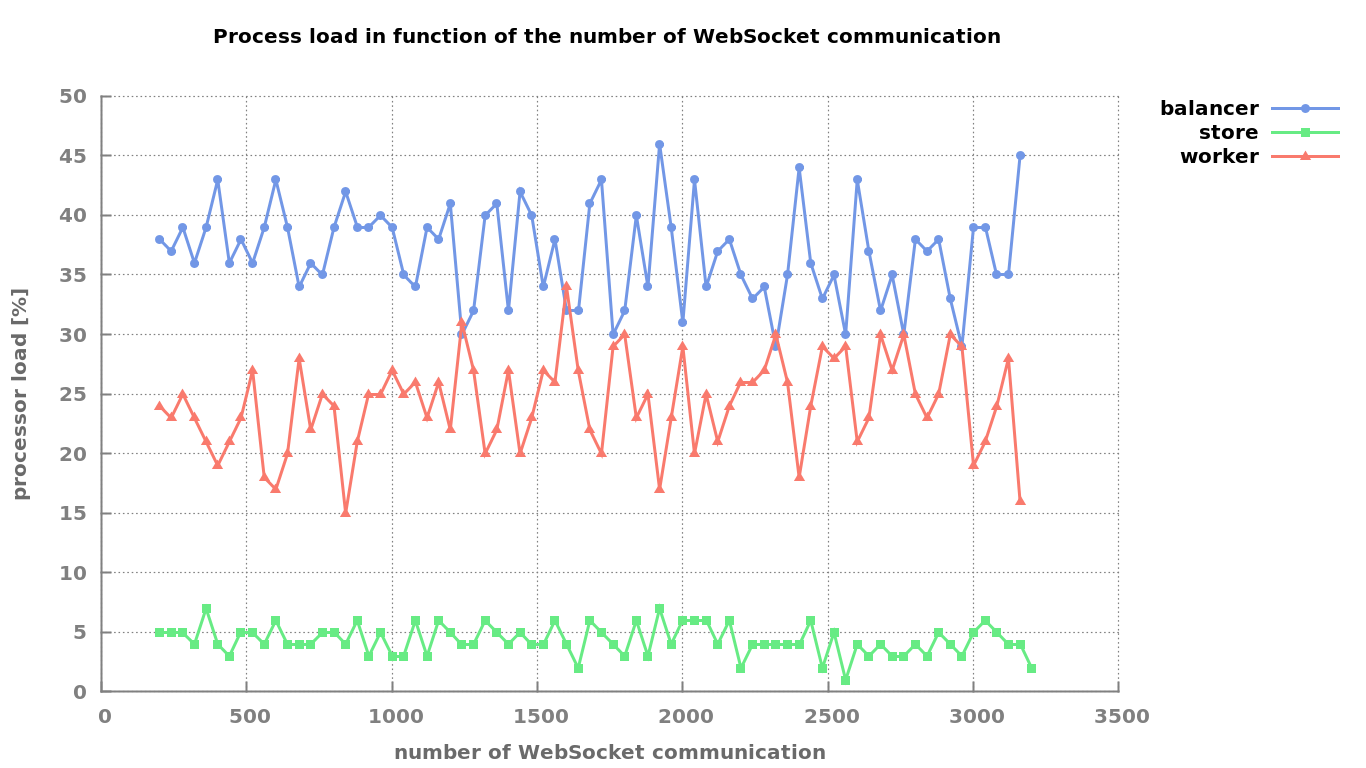
\includegraphics[width=\textwidth]{./Figures/WS_server_context.png}
	\caption[Contexting switching]{Context switching}
	\label{fig:context}
\end{figure}

At the first glimpse, anyone can immediately tell there is a problem with the server
graph. The Load seems to vary randomly at an average of 40\%. What really happens, is
that most WebSocket connections are dropped shortly after beeing created or they 
not even created. The problem is a single core needs to handle four threads. So each
time another application is called the context changes. The result is even worse case of 
a multi-procesor server, because threads then are balanced between processor. Threads 
are heavy weight units, moving them introduces consequent overheads.\\

to conclude, this experiment prooves SocketCluster is not aimed to be used with
project which imvolve more threads than available cores.\\

% --------------
% Fourth section
% --------------

\section{}


\textbf{Client code}

The client code used in all this part is the same. Two clients are used to
produce a maximum of 2400 WebSocket communications.


\begin{center}
  \begin{tabular}{ | l | l |}
  \hline
  \multicolumn{2}{|c|}{Parameters} \\
  \hline
    Instance type &  amazon ec2 m3.2xlarge\\ 
    Experiment time & 60 s \\
    Number of new communication created at each iteration & 20 \\
    Client creation period & 1 s \\
    Type of ping & random number \\ 
    Ping period & 2.5 s \\ 
    Number of clients & 2 \\
  \hline
  \end{tabular}
\end{center}


\begin{figure}[H]
	\centering
		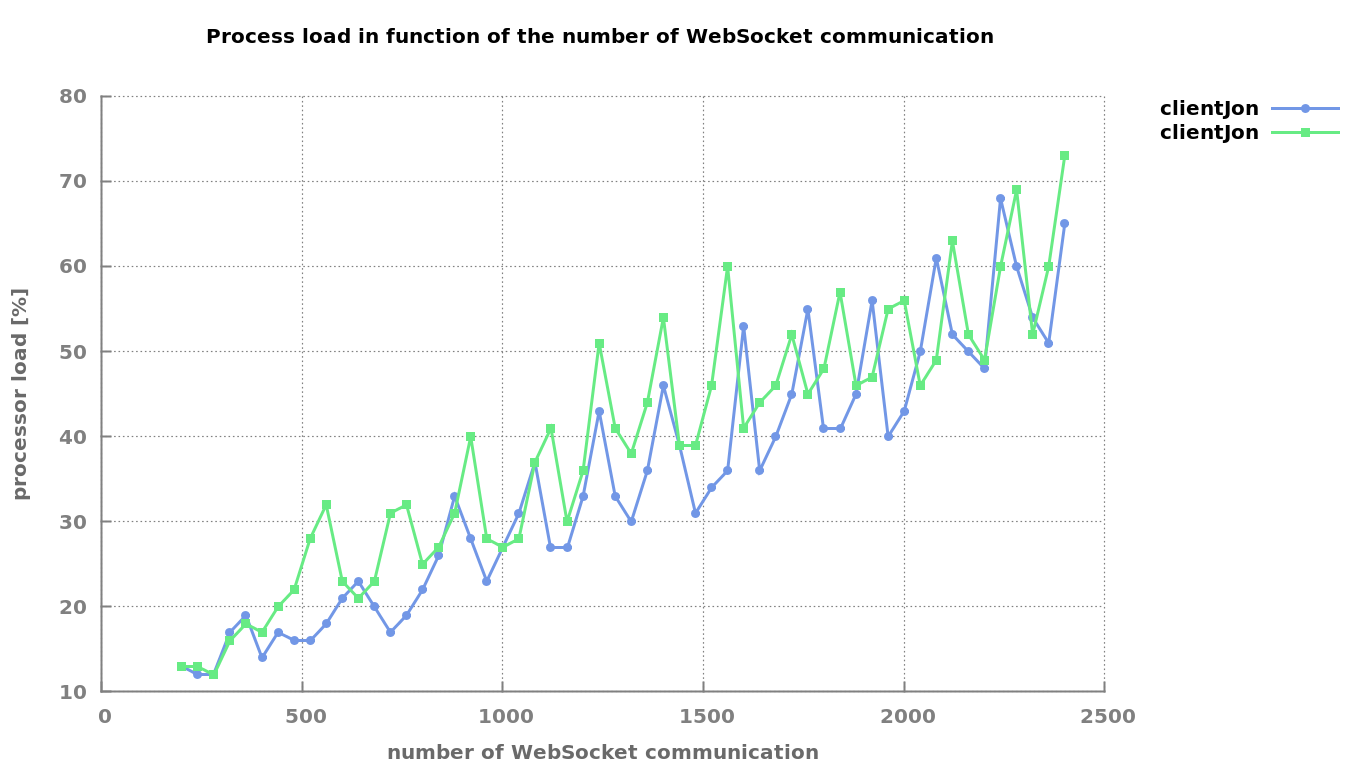
\includegraphics[width=\textwidth]{./Figures/WS_client_rising.png}
	\caption[Simple WebSocket client]{client code}
	\label{fig:WS_client_rising}
\end{figure}

\textbf{Server code}

The first test is run a server using a one store, one load balancer and one
worker.

\begin{figure}[H]
	\centering
		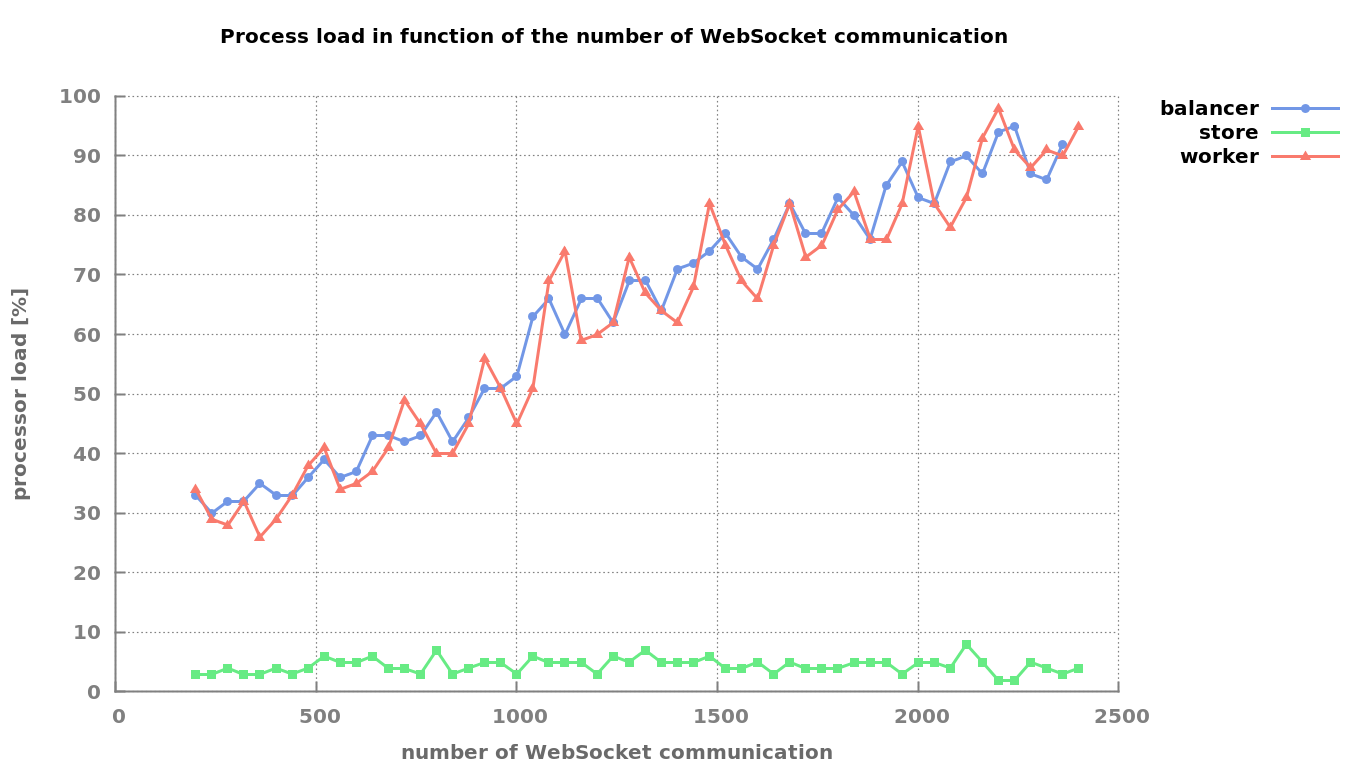
\includegraphics[width=\textwidth]{./Figures/WS_server_1rising.png}
	\caption[WebSocket server on three cores]{Server with 3 cores}
	\label{fig:WS_server_1rising}
\end{figure}

figure \ref{fig:WS_server_1rising} clearly shows the worker and loadbalancer
cores are almost used to their full extent. In order to handle more communication more
cores should be added. 

\begin{figure}[H]
	\centering
		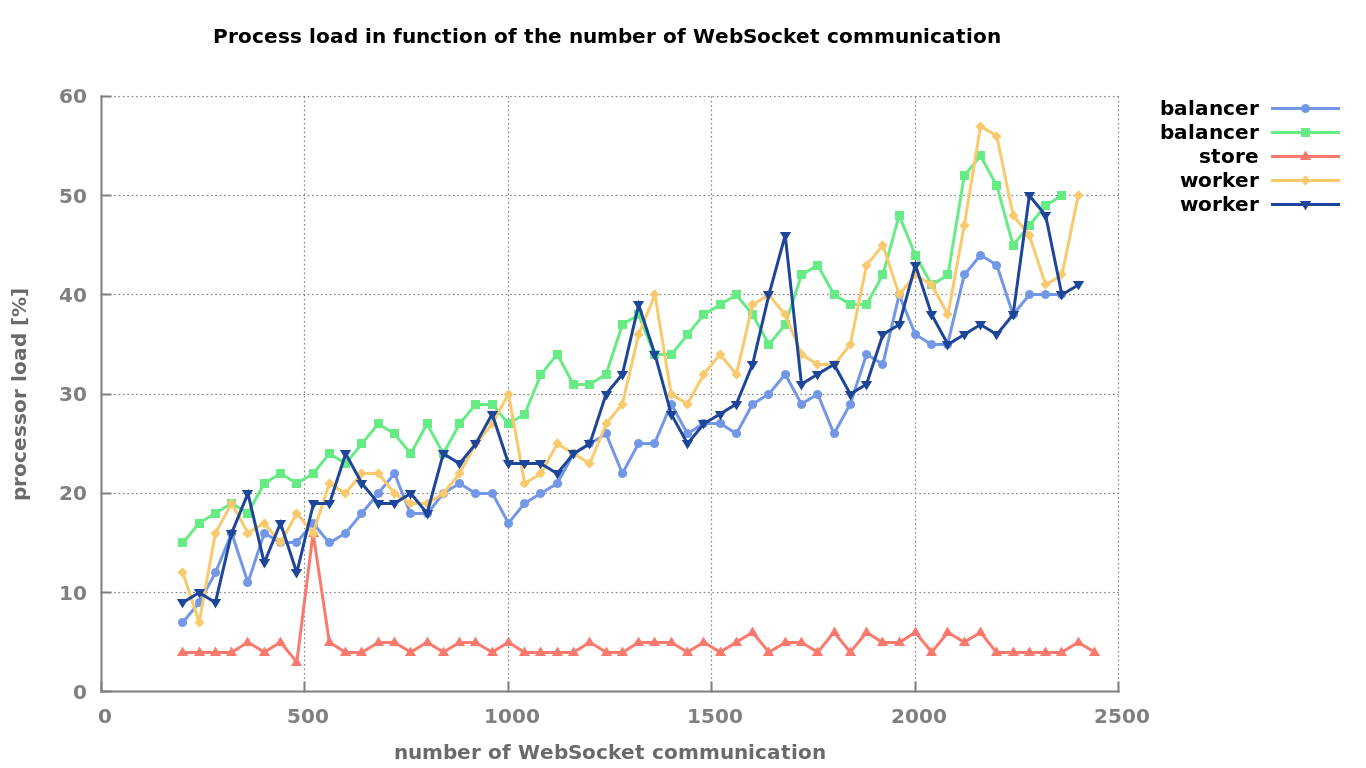
\includegraphics[width=\textwidth]{./Figures/WS_server_2rising.png}
	\caption[WebSocket server on five cores]{server with 5 cores}
	\label{fig:WS_server_2rising}
\end{figure}

In this experiment two more cores have been thrown to work. Load balancers and
workers nicely balance the work between themselves and the maximum load drops to 50\%.

\begin{figure}[H]
	\centering
		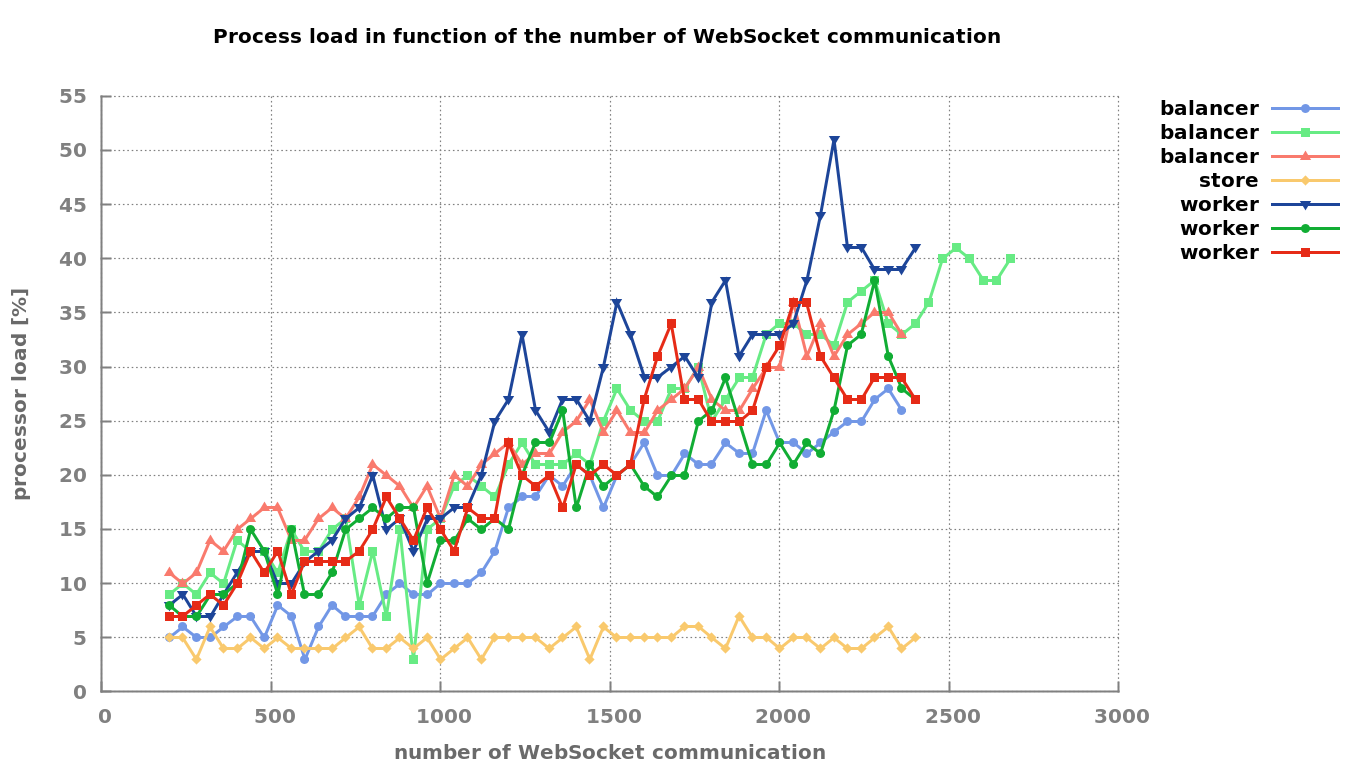
\includegraphics[width=\textwidth]{./Figures/WS_server_3rising.png}
	\caption[WebSocket server on seven cores]{server with 7 cores}
	\label{fig:WS_server_3rising}
\end{figure}

this last test is less conclusive. With a total of 3 cores for load balancers
and three for workers the processors load varies between 30\% and 50\%
depending on the task.\\

Adding too many cores is a waste of ressources, this stresses the importance of
finding a load balancer/worker/store ratio rule.


B] section most influence frequence pings / size message / number communications

c] General rule

load balancer / store / worker
 % Experiment 1

%\chapter{Conclusion} 
\label{Chapter5} 
\lhead{Chapter 5. \emph{Conclusion}} 

After studying the current landscape of research around WebSocket 
in a ditributed environment, this thesis focuses on the benchmarking 
of the node.js's real time engine SocketCluster.\\

SocketCluster is a promising library still actively under development.
It efficiently provides a highly scalable WebSocket server that make
use of all available CPU cores on an instance. It removes the limitation
of having to run Node.js code on single cores.\\

Experiments carried out on SocketCluster revealed two main limitations.  If
running on comparable hardware, a SocketCluster worker will be less efficient
then a basic engine.io implementation. Also SocketCluster efficiency
dramatically drops if run with more process then available cores because of
context switching.\\

Anyway, SocketCluster should be used in highly parallel environment and
therefore these limitations rarely appply. SocketCluster theoriticaly  enables
user to scale an application vertically  without limits. N being the number of
cores the server has, SocketCluster has been prooved to be at least
$\frac{N}{2}$ more efficient then a basic node.js implementation.  As the
number of cores rises, it looks like the performance could be slightly better
then $\frac{N}{2}$. The load balancers begins to missbehave and performances
are limitted by a few overloaded load balancers. However, it is probably only a
question of time until a patch fixes this issue.\\

While benchmarking SocketCluster, useful SocketCluster features were
considered.  System administrator could benefit from a realtime monitoring tool
to check the state of each threads and thus help them manage the size of the
cluster. The monitoring tool could even be linked with an algorithm to
automatically append or delete threads.  SocketCluster would then be an autonom
entity. Scaling on its own without any human interaction.\\



 % Experiment 2

%\input{./Chapters/Chapter6} % Results and Discussion

%\input{./Chapters/Chapter7} % Conclusion

%% ----------------------------------------------------------------
% Now begin the Appendices, including them as separate files

\addtocontents{toc}{\vspace{2em}} % Add a gap in the Contents, for aesthetics

\appendix % Cue to tell LaTeX that the following 'chapters' are Appendices

\chapter{SocketCluster}
\label{SocketCluster}
% \lhead{Appendix A. \emph{SocketCluster}}
\section{Simple ping-pong exchange}
\textbf{Client code}


This is an example of a WebSocket client code spread on all available cores.
New clients are spawned every \texttt{numberClientsEachSecond}. Thereafter,
every \texttt{intv} each clients sends a ping event cast to a Javascript JSON
object.

\begin{figure}[H]
	\centering
		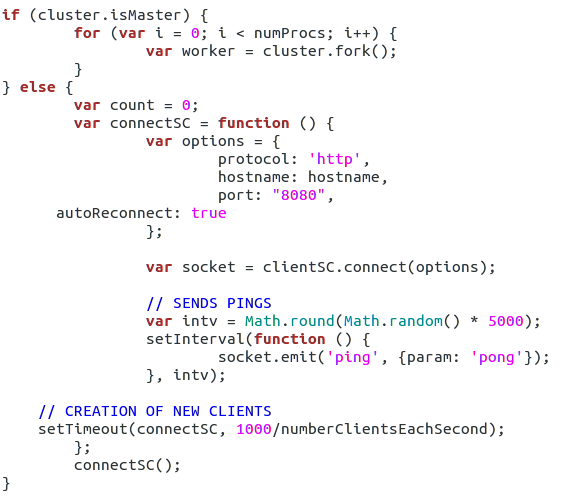
\includegraphics[width=0.7\textwidth]{./Figures/WS_client_simplePing.png}
	\caption[WS_client_simplePing]{Pings from client}
	\label{fig:WS_client_simplePing}
\end{figure}

To best simulate clients interaction with a websocket server, new sockets are
created at random intervals \texttt{intv = Math.round(Math.random()*5000)}.

\textbf{Server code}

The server listens for pings event and answers back with pongs event. In this
case the pong event is an integer counting the number of pings this particular
worker had during the whole experiment.

\begin{figure}[H]
	\centering
    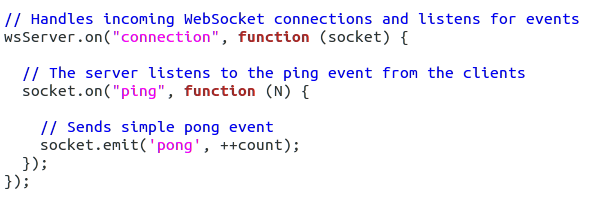
\includegraphics[width=0.9\textwidth]{./Figures/WS_server_simplePong.png}
	\caption[WS_server_simplePong]{Server answering with pongs}
	\label{fig:WS_server_simplePong}
\end{figure}

\section{File transfer}

\textbf{Client code}

In this example, the goal is to exchange a file using the WebSocket protocol.
For this purpose, the node.js \texttt{delivery} library is used.

New clients are created on the same model as the previous exmample. Each new
client is stored in the \texttt{clients} array. Each clients are also
perdiodically sending pings. The only add on is the \texttt{map} function to
enable the each socket to retrieve the document sent by the server. 

\begin{figure}[H] \centering
  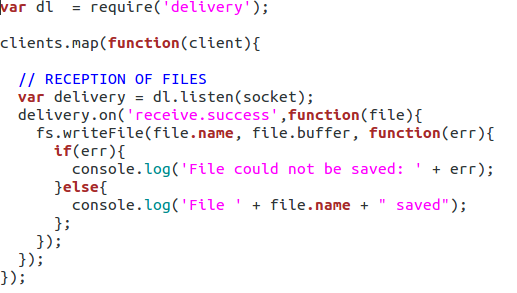
\includegraphics[width=0.9\textwidth]{./Figures/WS_client_delivery.png}
\caption[WS_client_fileTransfer]{Clients receptionning files} 
\label{fig:WS_client_fileTransfer}
\end{figure}

\textbf{Server code}

The server listens for pings. And sends back a file, \texttt{foo.txt} in this
example.

\begin{figure}[H]
	\centering
    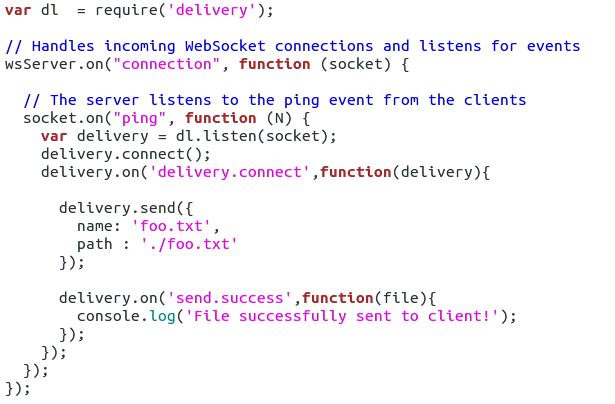
\includegraphics[width=0.9\textwidth]{./Figures/WS_server_delivery.png}
	\caption[WS_server_simplePong]{Server sending files}
	\label{fig:WS_server_simplePong}
\end{figure}
	% Appendix Title

%\chapter{Engine.io}
\label{engine}
% \lhead{Appendix A. \emph{SocketCluster}}

This appendix gives the code used to create a simple engine.io server and
client. Comparaison with SocketCluster code in appendix \ref{SocketCluster} 
shows the difference between both implementation is small. 

In fairness, SocketCluster API is very close to engine.io.

\textbf{Client code}

\begin{figure}[H]
	\centering
		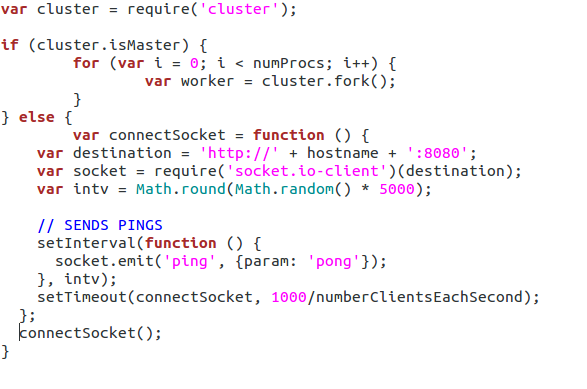
\includegraphics[width=0.9\textwidth]{./Figures/engine_client_simplePong.png}
	\caption[Engine.io client code]{Pings from client}
	\label{fig:engine_client_simplePing}
\end{figure}


\textbf{Server code}


\begin{figure}[H]
	\centering
    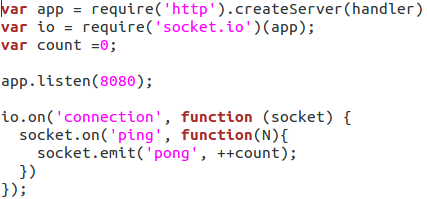
\includegraphics[width=0.7\textwidth]{./Figures/engine_server_simplePing.png}
	\caption[Engine.io server code]{Server answering with pongs}
	\label{fig:engine_server_simplePong}
\end{figure}

 % Appendix Title

%\chapter{Real time throughout check}
\label{indexHTML}

By inserting the following script in \texttt{index.html} the browser will
display in realtime the number of pings received by a WebSocket server.

\begin{figure}[H] \centering
  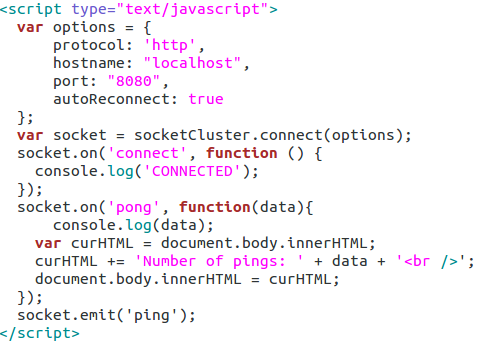
\includegraphics[width=0.8\textwidth]{./Figures/index_script.png}
\caption[index_script]{Modification to \texttt{index.html}}
\label{fig:index_script} \end{figure}

All it does is emitting a ping, then listening to the pong event and displaying
it directly in the html page. The pong payload as can be seen in
\ref{fig:WS_server_simplePong} is \texttt{count}, an integer increamented each
new ping.
 % Appendix Title

\addtocontents{toc}{\vspace{2em}}  % Add a gap in the Contents, for aesthetics
\backmatter

%% ----------------------------------------------------------------
\label{Bibliography}
\lhead{\emph{Bibliography}}  % Change the left side page header to "Bibliography"
\bibliographystyle{unsrtnat}  % Use the "unsrtnat" BibTeX style for formatting the Bibliography
\bibliography{Bibliography}  % The references (bibliography) information are stored in the file named "Bibliography.bib"

\end{document}  % The End
%% ----------------------------------------------------------------
